% !TEX encoding = UTF-8 Unicode
% !TEX root = ../../Masterthesis.tex

\chapter{neo-Riemannian Theory}\label{ch:nrt}
% \morefloats

\newthought{Traditional} tonal harmonic analysis is designed to handle the sonorities constitutionalized in the Baroque and Classical eras. The idea is that any given chord tells something about where it stands in relation to the chord preceding it. Put rather bluntly every chord, given a long enough chain, could be interpreted as a dominant or a part of a cadence heading for, or avoiding a tonic. While this is perfectly adequate for most diatonic-based music, chromatic music that is triadic but not altogether unified under a diatonic rule, does serve a challenge for traditional functional analysis. \acf{nRT}\footnote{The abbreviation is nRT, with a small \textit{n} pointing to the fact that this maybe has grown beyond the \textit{''neo''} tag. \textquote[{\cite[1]{Lehman_2015}}]{(...)this no-longer so ``neo'' theoretical system.}} was developed to handle this issue.

Let us examine the following:

\begin{figure*}[h!]
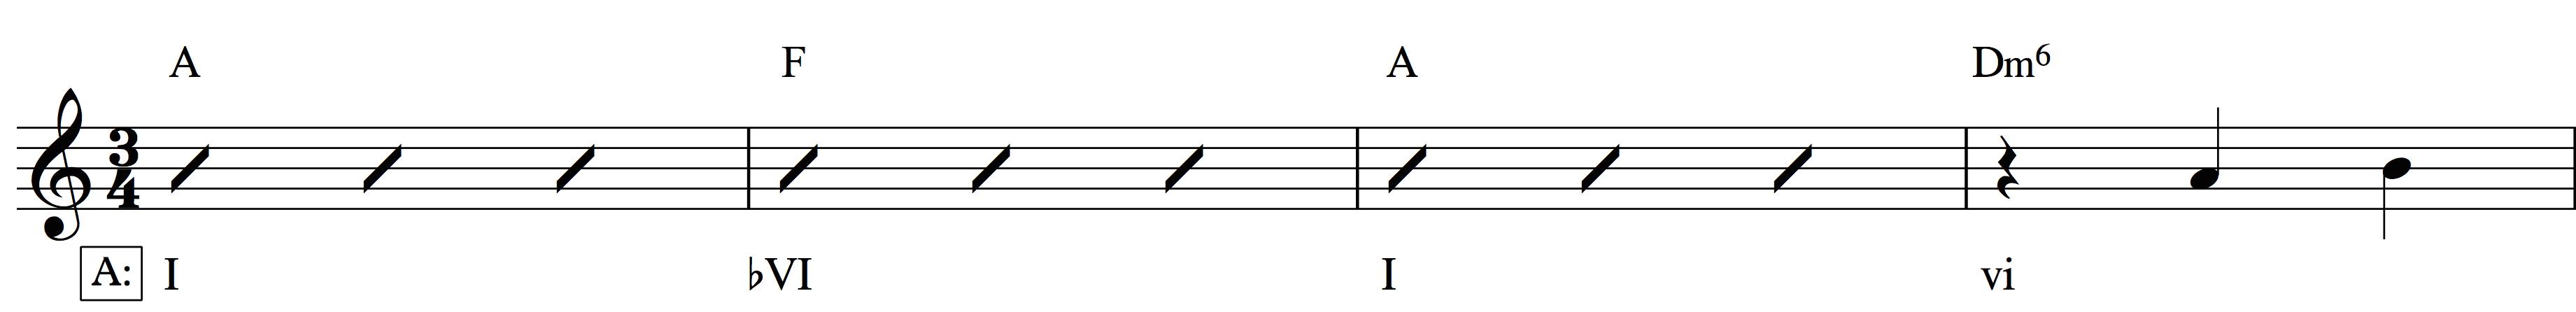
\includegraphics[width=\linewidth]{Ilia_Theme_1}
	\caption{Ilia's Theme 1}
	\label{Ilia_Theme_1}
	%\setfloatalignment{b}
\end{figure*}

\begin{figure}[h!]
\center
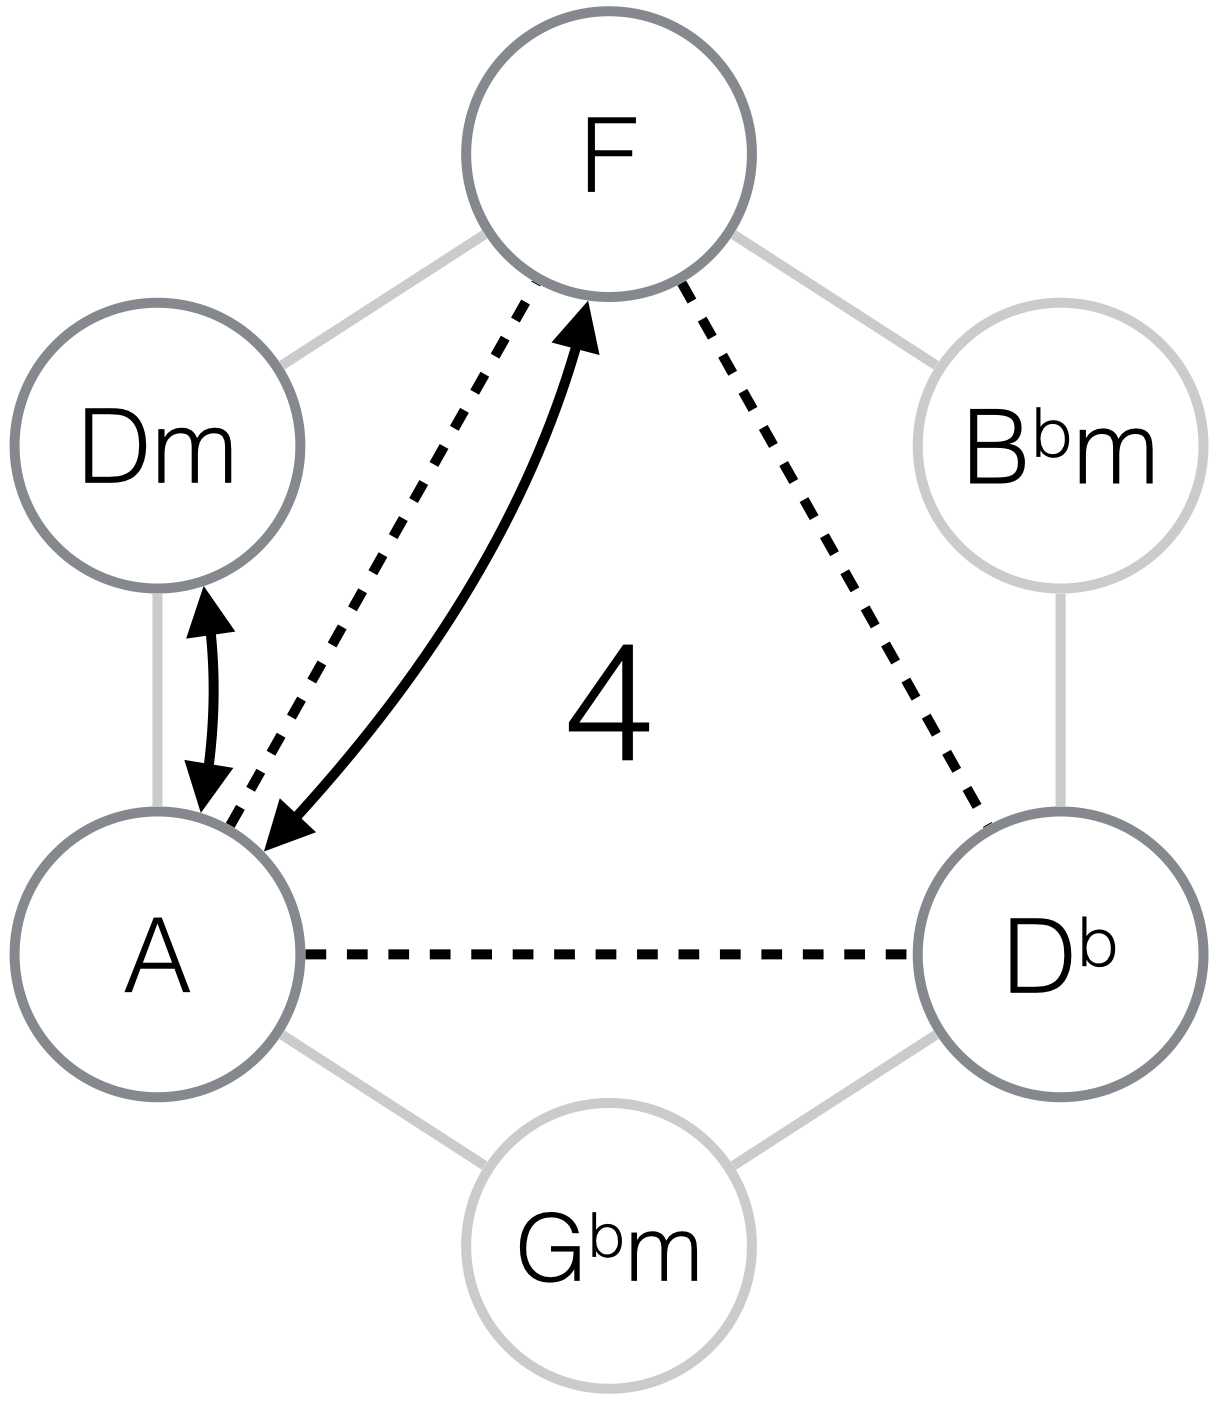
\includegraphics[width=0.5\linewidth]{Ilia_theme_1_nrt}
	\caption{Ilia's Theme m. 1-4}
	\label{Ilia_theme_1_nrt}
	\setfloatalignment{b}
\end{figure}

\noindent This show an excerpt from Goldsmith ``Ilia's Theme'' from \ac{ST:TMP}\footnote{See the complete sheet music on page \pageref{Ilias_Theme}}. If one where to analyze this using traditional tools we immediately run into a problem: What to define as the tonic? If we assume A, then F becomes \(\flatx{VI}\), and this makes sense because the \chord{Dm}{6} makes what we can identify as a \textit{Hollywood Cadence} \(({iv}\Rightarrow{I})\). If we assume F, then A becomes \(III\) and the \chord{Dm}{6} becomes \(vi\) which also makes sense. Within the context of a circle of fifths it makes no sense at all as it fits neither heads or tail of the Tonic, Subdominant, Dominant triangle for neither A nor F. So right from the get-go we have two possible candidates for a tonic. The same dichotomy of tonality continues throughout the first part of the cue.

\begin{figure*}[h!]
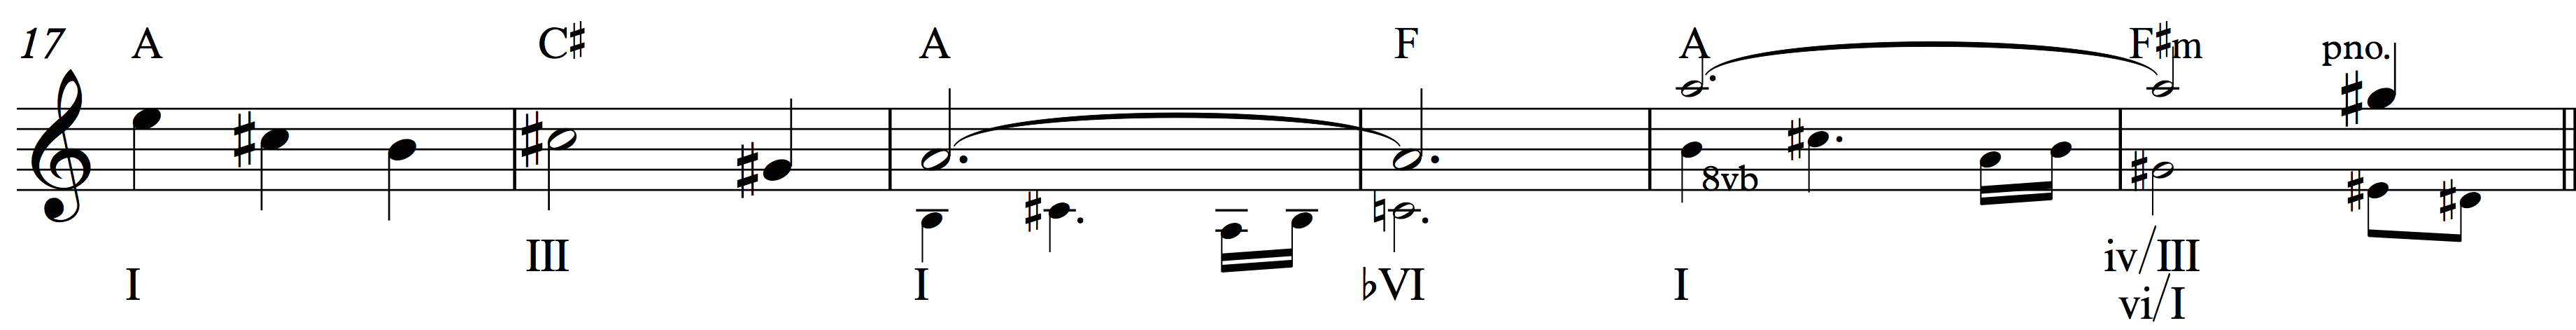
\includegraphics[width=\linewidth]{Ilia_Theme_2}
	\caption{Ilia's Theme 2}
	\label{Ilia_Theme_2}
	\setfloatalignment{b}
\end{figure*}

In \textbf{m.17-22}, figure \ref{Ilia_Theme_2}, we see some movement that further could indicate A as tonic seeing that we have both \(III/A\) and \(vi/A\), acting internally as \(V/vi-i/vi\) and prepare us for \textbf{m.23} where the yet another juxtaposition seems to unfold: figure \ref{Ilia_Theme_3}.

\begin{figure*}[h!]
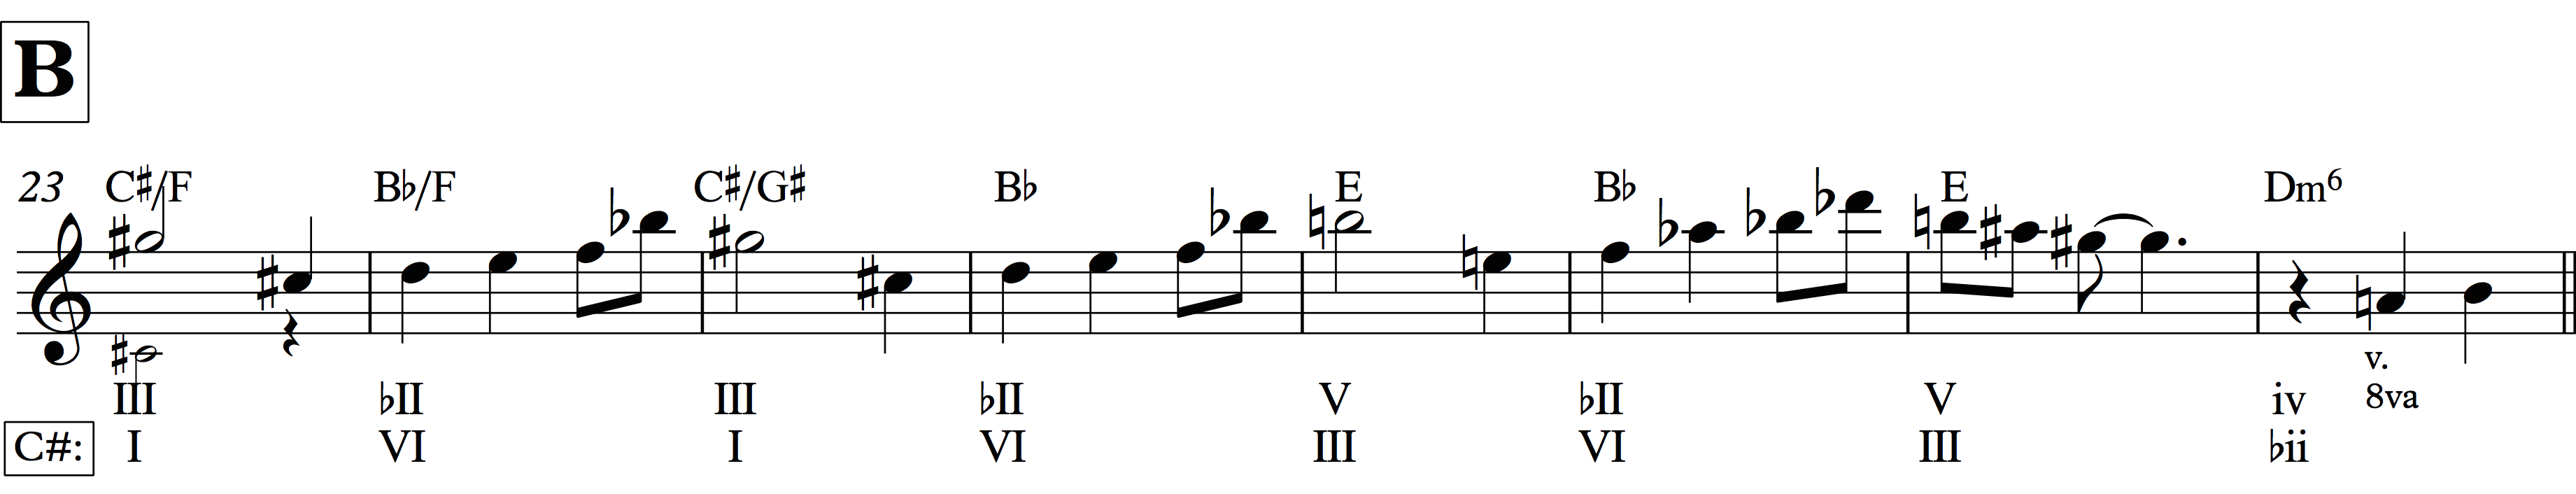
\includegraphics[width=\linewidth]{Ilia_Theme_3}
	\caption{Ilia's Theme 3}
	\label{Ilia_Theme_3}
	%\setfloatalignment{b}
\end{figure*}

Now \dflat/\ciss revolves around \bflat and then \bflat and E before ending on \chord{Dm}{6}. The internal logic does not comply with the ordinary predictions we can make from \(I-IV-V\) and its children. If we, however, apply the logic from transformational analysis we get to another picture. 

We can make a circle of chords based on different transformations then that of the circle of fifths, in this case major thirds, we can see some sort of logic underpinning the progression. If we assume A as the \textit{tonal centre} we can see that by moving from \(I\) to \(iv\) making it the new \(vi\) we get the formula: \({I}\Rightarrow{iv/vi}\) thus producing a circle of thirds. This circle is know as a \textbf{NR\(_{4}\)} circle and I will explain these circles in greater detail further down the chapter. With this we have a model that explains the majority of the first part. 

\begin{figure}[h!]
\center
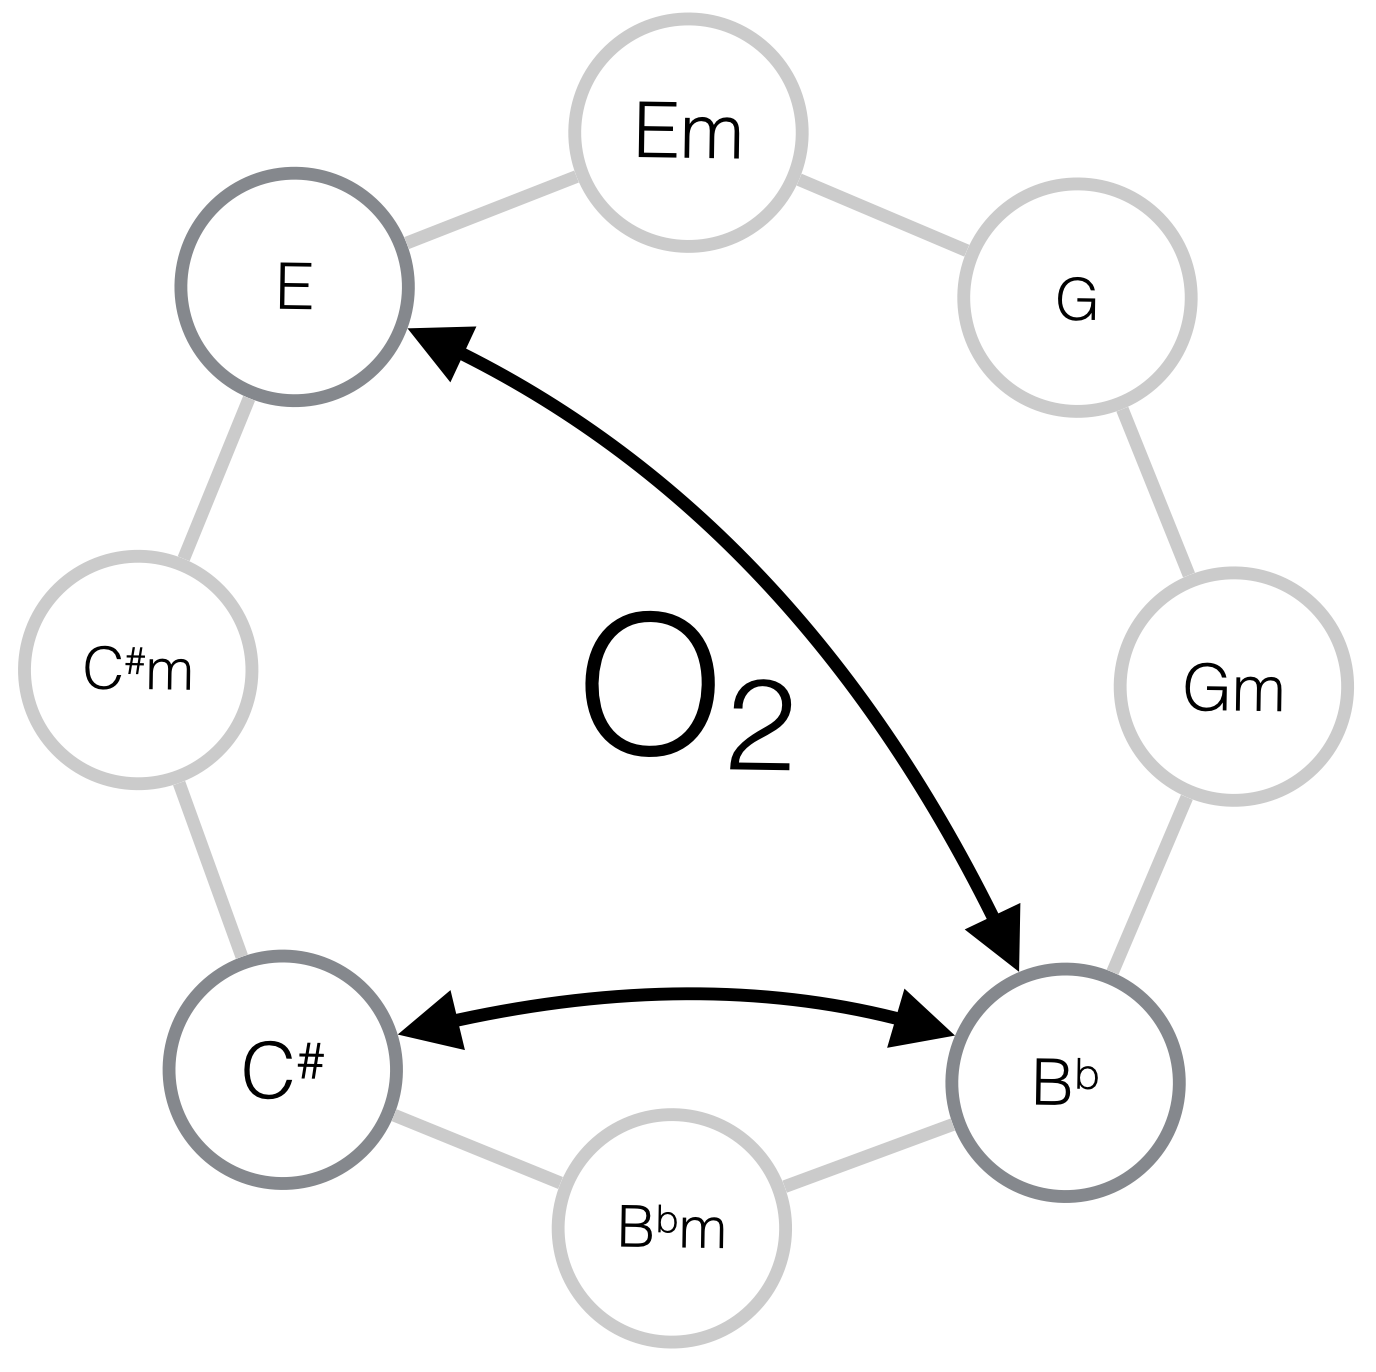
\includegraphics[width=0.55\linewidth]{Ilia_theme_2_nrt}
	\caption{Ilia's Theme, m.23-29}
	\label{Ilia_theme_2_nrt}
	\setfloatalignment{b}
\end{figure}

With the second part, figure \ref{Ilia_Theme_3}, we can build a figure, (\ref{Ilia_theme_2_nrt}) using the same logic; a \textit{hexatonic} circle of thirds that we can see is in relation with the movements in \textbf{m.23-30} where the tonal centre is \ciss from which it is possible to build a \textit{octatonic} circle of minor thirds, and thus making the relationship between \bflat and E not so far fetched as one might think. To top it of, one might make a compound diagram that shows that the two parts are indeed related thanks to the common chord \ciss. The conclusion from this short example is that the chord structure is largely govern by thirds and that \textbf{m.1-22} (Letter A) and B has a common root.

\begin{figure}[h!]
\center
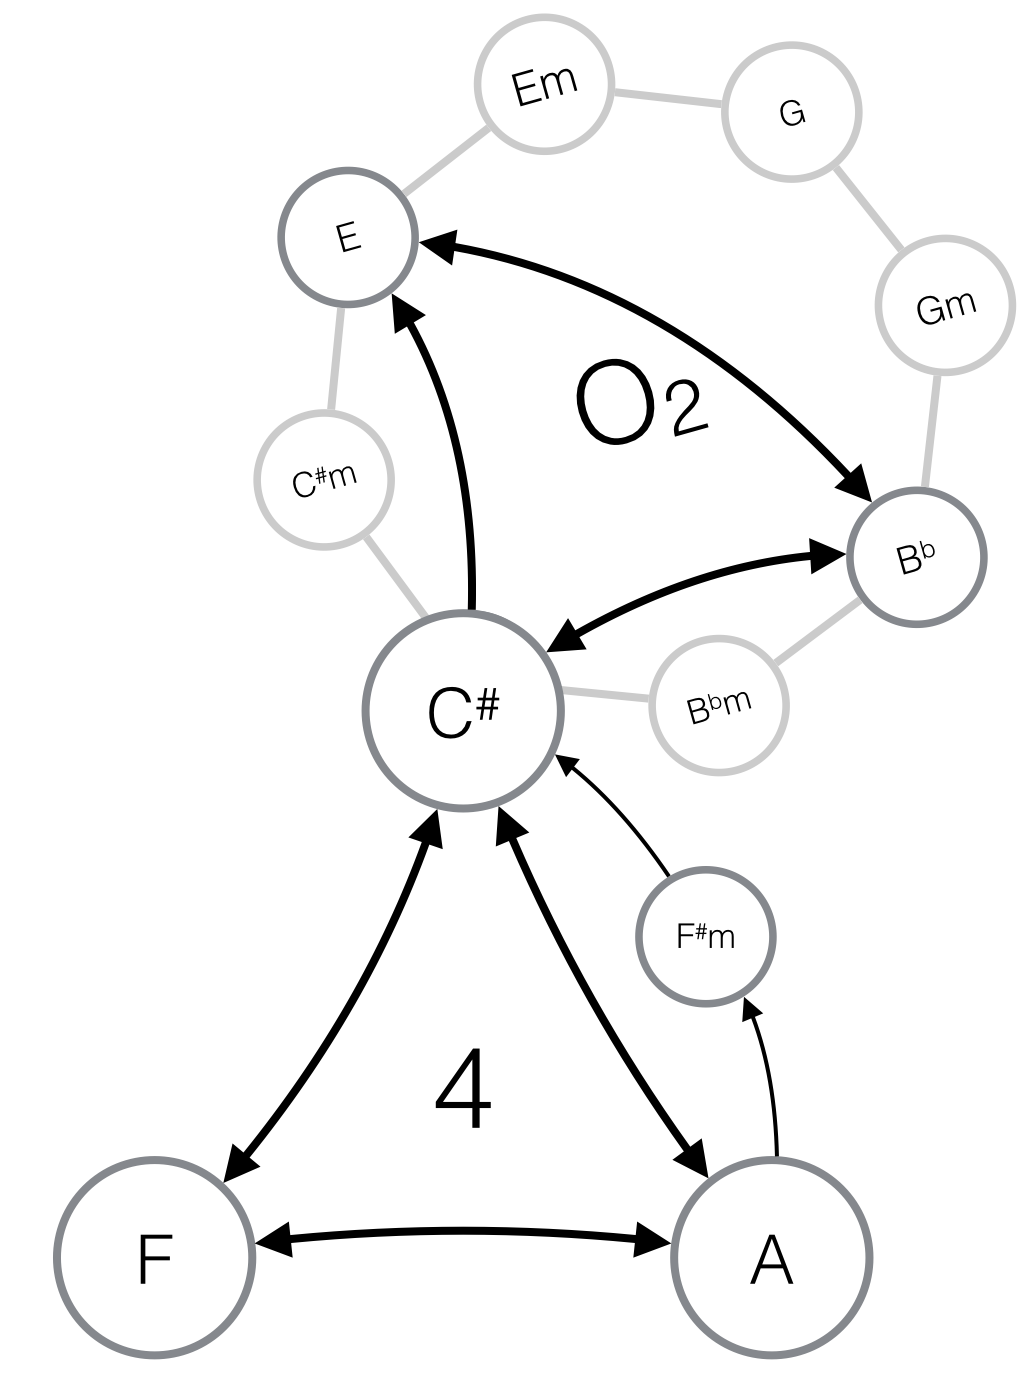
\includegraphics[width=0.55\linewidth]{Ilia_theme_3_nrt}
	\caption{Ilia's Theme, m.17-29}
	\label{Ilia_theme_3_nrt}
	%\setfloatalignment{b}
\end{figure}

\ac{nRT} originates from David Lewin. He wrote an essay in 1987 titled: \textit{``Generalized Musical Intervals and Transformations''}\footnote{\textcite{lewin_generalized_2007}. I suggest reading Richard Cohn's introduction to neo-Riemannian theory, \parencite{cohn_introduction_1998} for those of historically inclined as I will not cover the historical backdrop in this thesis.} that laid the premise for this type of transformational analysis. According to Cohn it was created to serve the analytical needs of nineteenth century music. Film music tonality has a lot of commonality with nineteenth century tonality in that the tonality is mostly tonal, but ununified\footnote{\textcite[p.2]{cohn_introduction_1998}}, i.e. not bound by a diatonic scale. Since Lewin's essay where published, the theory has gained traction with the likes of Richard Cohn\footnote{\textcite{cohn_maximally_1996}} and Frank Lehman\footnote{\textcite{lehman_reading_2012}}, among others. Lehman's work on how to apply \textit{transformational analysis}, as this branch of theory is called, to film music is what has enabled me to do this thesis.

\begin{figure*}
\center
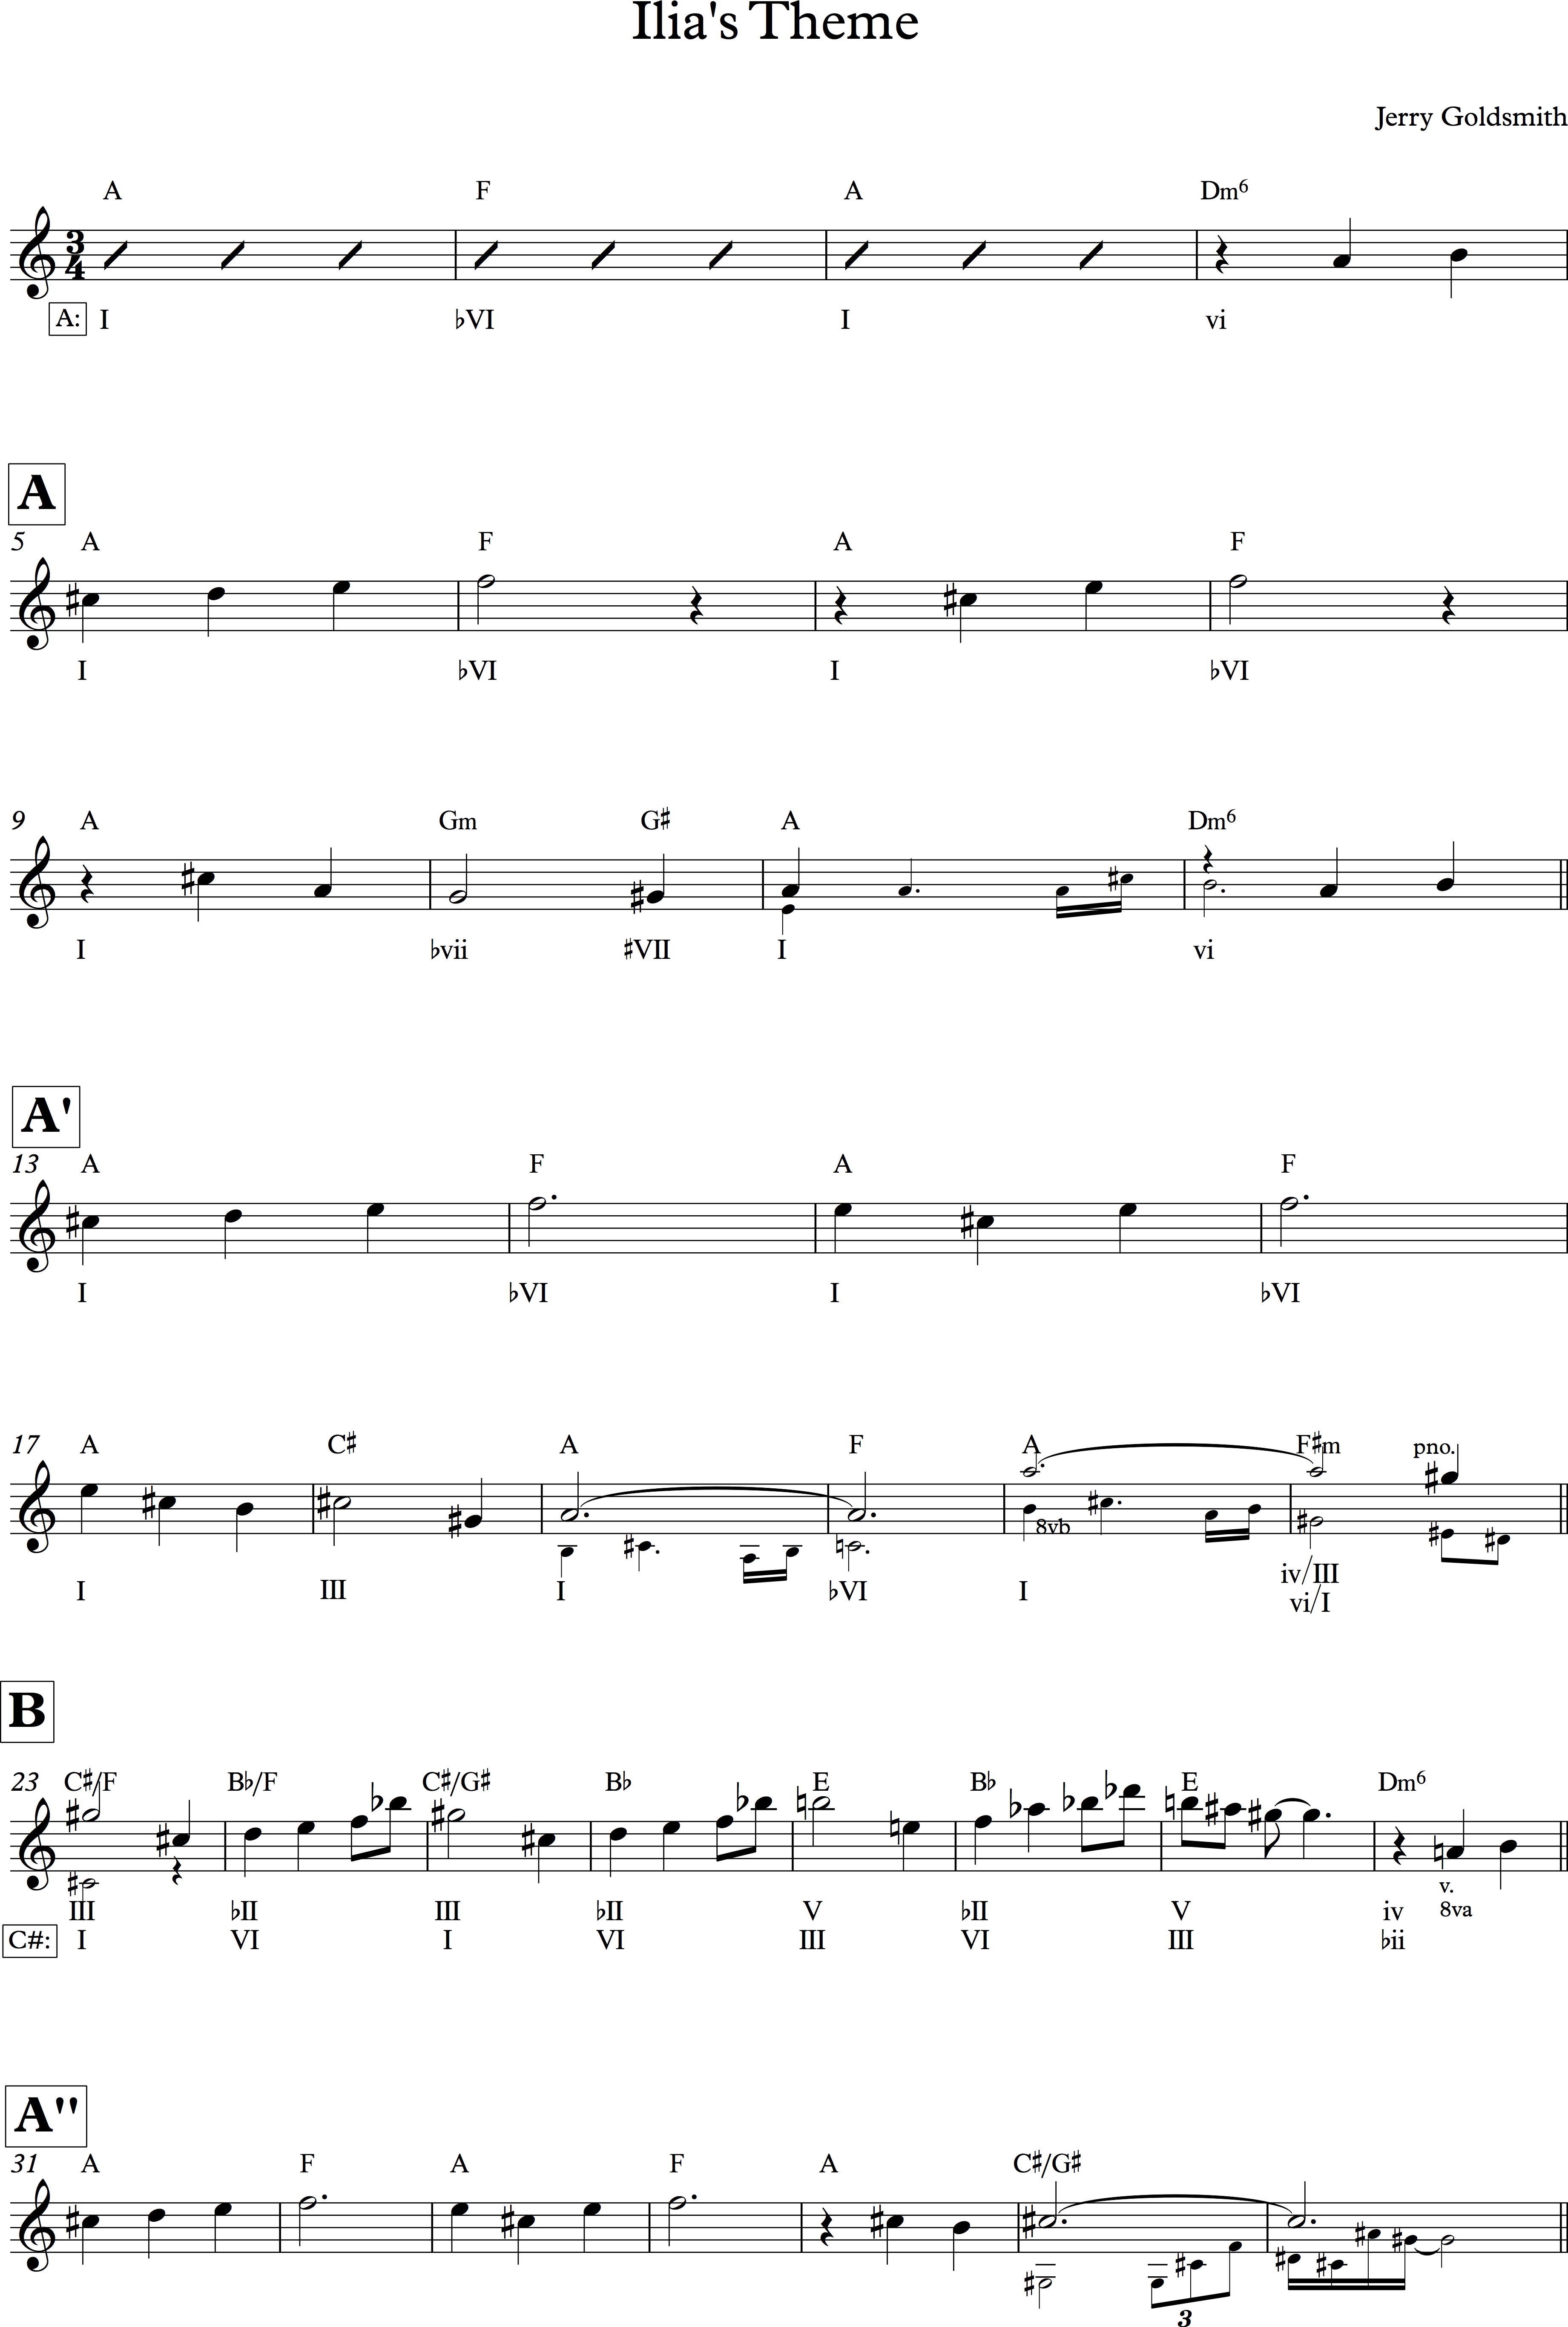
\includegraphics[width=\linewidth]{Ilias_Theme}
	\caption{Ilia's Theme}
	\label{Ilias_Theme}
	\setfloatalignment{b}
\end{figure*} 

\begin{marginfigure}
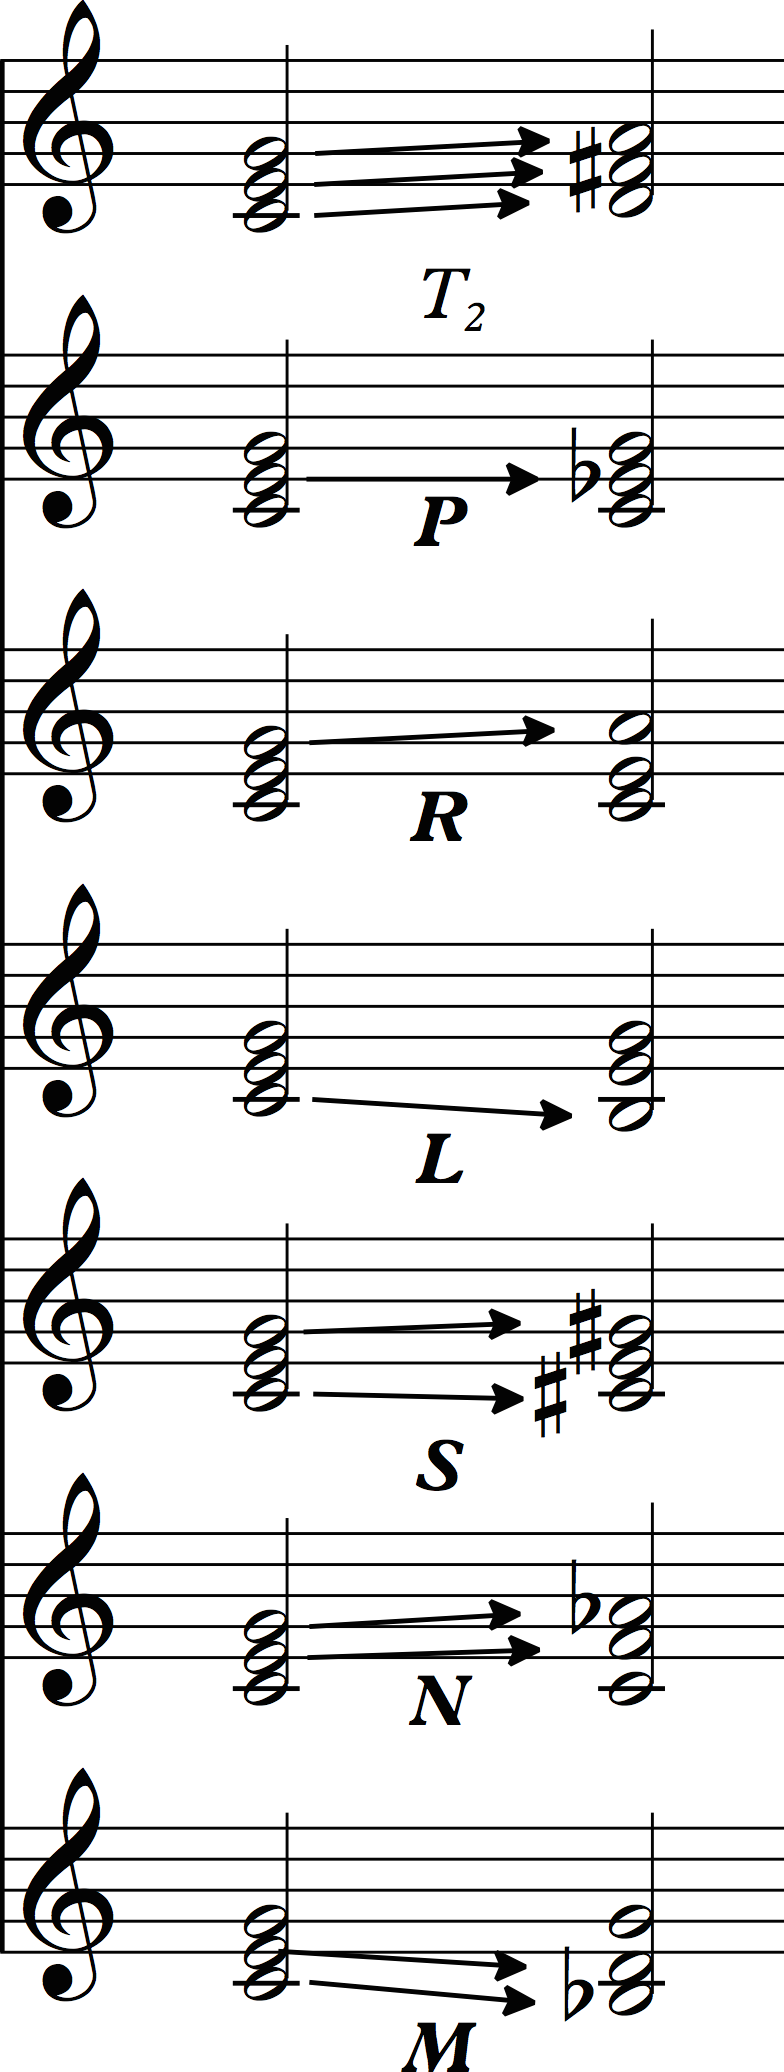
\includegraphics[width=0.7\linewidth]{PRL}
\caption{Basic NRT operators}
\label{fg:prl}
\end{marginfigure}

The main idea of \ac{nRT} is to look at harmonic relations without necessarily relating to a tonic. It does so by looking at how one state changes into another, i.e. \textit{transforms}. It excels as a tool to look for patterns in harmonic progressions otherwise obscured. It is a bit like \textit{Schenker graphs}, but unlike Schenker, \ac{nRT} does not need to work around functional analysis. It does so with tools that look at how a triad \textit{transforms} from one to another. Broken down to its bear essentials \ac{nRT} has three operators that transforms a triad to something else. These are \textbf{(P)arallel}, \textbf{(L)eittonwechsel} and \textbf{(R)elative}. Each operator works both ways; when you have executed [operation] it works in reverse as well. 
\textbf{P} displaces the non-\textit{ic5} pitches in a triad, i.e moves the third between minor and major. For the sake of examples, we assume the first chord in the transformation is \(I\); ergo, in Schenkerian terms it would look like this: \({I}\Leftrightarrow{i}\). 
\textbf{L} displaces non-\textit{ic3} pitches, i.e. the unison in major or the fifth in minor: \({I}\Leftrightarrow{vi}\).
\textbf{R} Displaces the non-\textit{ic4} pitches, i.e the fifth in major and unison in minor: \({I}\Leftrightarrow{vi}\). 
By combining these three operators, it is possible to create \textit{compound operators} and, as such, maneuver from and to each major and minor triad in the 12 tone scale. However, to address some of the more common maneuvers, I will be using a couple of other tools as well. 
\textbf{(S)lide}\footnote{Introduced by \citealt{lewin_generalized_2007}.}, a shorthand for \textbf{L}, \textbf{P} and \textbf{R}, displaces \textit{ic5} pitches, i.e. they move both the prime and fifth: \({I}\Leftrightarrow{\flatx}{ii}\). 
\textbf{(N)ebentonverwandt}\footnote{From Weitzmann via \citealt{lehman_reading_2012}.} displaces the \textit{ic3} pitches, i.e. \({I}\Leftrightarrow{iv}\).  
\textbf{(M)odelverwant}\footnote{Introduced by Frank Lehman in his 2012 dissertation.} displaces ic4 pitches, i.e. \({I}\Leftrightarrow{v}\). I will use \(T_{n}\) to indicate a direct transposition. In addition to the \ac{nRT} operators, I will use diatonic functions as well, indicating \textbf{Tonic}, \textbf{(Dom)inant}, \textbf{(Subd)ominant}, \textbf{(Med)iant} and \textbf{(Subm)ediant} 

\begin{table}
	\small
	\begin{tabularx}{\textwidth}{lll}
		\textbf{Operators}                              				& \textbf{Example}                     	\\ 
		\toprule
		\(T_{n}\): Transpose by \(_{n}\) semitones.    		& \textbf{\(T_{2}\)}\(\Rightarrow\)C=D	\\
		\textbf{P}arallel: Displace non-ic5 pitch       		& \textbf{P}\(\Rightarrow\)C=Cm      	\\
		\textbf{L}eittonwechsel: Displace non-ic3 pitch 		& \textbf{L}\(\Rightarrow\)C=Em      	\\
		\textbf{R}elative: Displace non-ic 4 pitch      		& \textbf{R}\(\Rightarrow\)C=Am      	\\
		\textbf{S}lide: Displace ic5 pitches            			& \textbf{S}\(\Rightarrow\)C=\cissm 	\\
		\textbf{N}ebentonverwandt: Displace ic3 pitches 	& \textbf{N}\(\Rightarrow\)C=Fm      	\\
		\textbf{M}odelverwant: Displace ic4 pitches     		& \textbf{M}\(\Rightarrow\)C=Gm     	\\ 
		\textbf{T}onic								& Chord on scale degree \(\hat{1}\) 	\\
		\textbf{DOM}								& Chord on scale degree \(\hat{5}\)	\\
		\textbf{SUBD}								& Chord on scale degree \(\hat{4}\)	\\
		\textbf{MED}								& Chord on scale degree \(\hat{3}\)	\\
		\textbf{SUBM}								& Chord on scale degree \(\hat{6}\)	\\
		\bottomrule
	\end{tabularx}  
	\caption{Transformational Inventory}
    	\label{tb:transformational_inventory}
\end{table}

%-----------------------------------------------------------------------------
% NRT and Symmetry
%-----------------------------------------------------------------------------
\begin{figure*}[h!]
\texttt{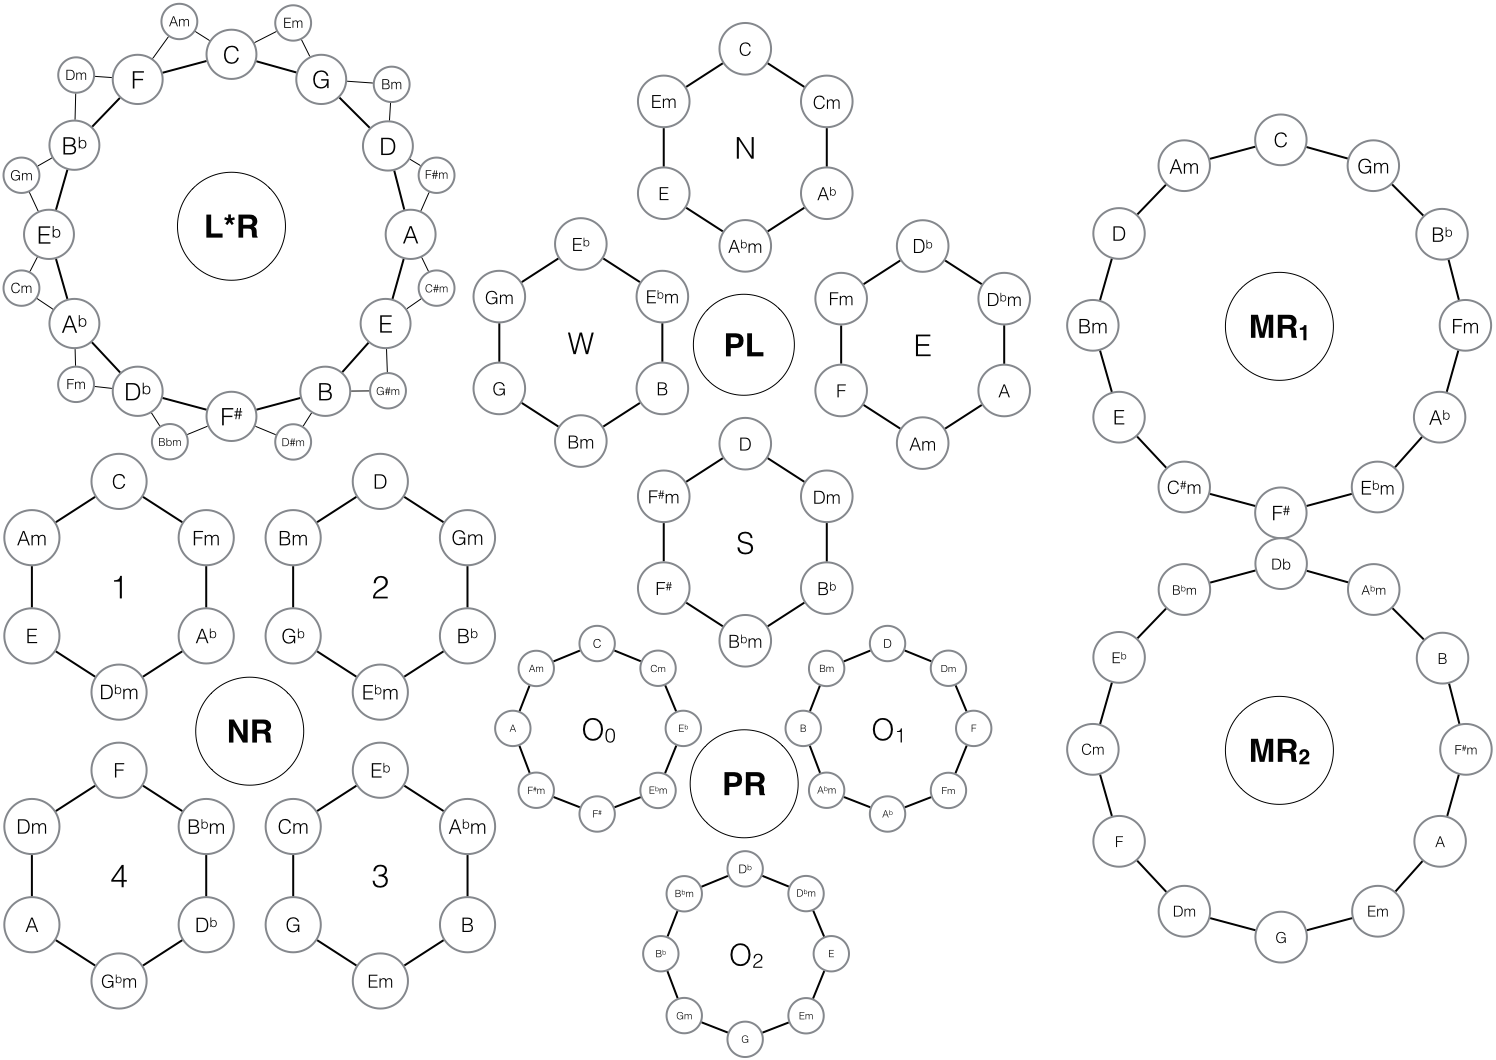
\includegraphics[width=\linewidth]{nrt_circles}
}\caption{neo-Riemannian circles}
\label{fg:nrt_circles}
\end{figure*} 

\section{Symmetry}
Just as we build circles of fifths (\textbf{L\(\cdot\)R}), we can do the same with different combinations of operators, e.g. \textbf{NR}, \textbf{PL}, \textbf{PR} and \textbf{MR}\footnote{It is possible to build other circles, but these are the ones I will use in this thesis}. These circles are what we call \textit{networks}. Each network consists of \textit{nodes} that represent a chord. A collection of networks is called a \textit{hyper system}, for instance, a \textit{hyper octatonic system}. Any given network has a unique name that mirrors the way they were created: \textbf{LR}, \textbf{NR\(_{1-4}\)}, \textbf{PL\(_{n,e,s,w}\)}. \textbf{PR O\(_{0-2}\)} and \textbf{MR\(_{1-2}\)}. In the case of \textbf{NR} and \textbf{PL}, we call them hexatonic networks because they consists of six nodes. It takes four networks to cover the entire major/minor cycle. \textbf{PR} is octatonic and uses three networks to fill the entire major/minor cycle. The \textbf{MR} network uses twelve nodes and requires two networks to complete the entire major/minor cycle. When a progression follows only a progression exclusively in one network, I call it a ``\textit{forced progression}'' and when a progression moves from one network to another, regardless of its parent, it is called a network modulation. In my analysis, these networks will always be displayed with their designators, but not necessarily the parent, for instance \textbf{PL}. Figure \ref{fg:nrt_circles} gives an overview over the networks I will be using. 

\marginnote[-5cm]{The heaxtonic \textbf{PL}, \textbf{PR} and octatonic \textbf{PR} networks are borrowed from Lehman and Lewin's papers and follow the designators used by them.}

	
%-----------------------------------------------------------------------------
% nRT Augmented chords
%-----------------------------------------------------------------------------

\section{Augmented Chords} 

\ac{nRT} was made to address major and minor triads and does so quite brilliantly. It does not, however, handle augmented chords at all. The question thus presents itself: How are augmented chords to be dealt with? One approach is, simply, to indicate that something has happened which could be interpreted with transformational glasses. Frank Lehman postulates an asterisk, \textbf{*}\parencite{lehman_reading_2012}, when dealing with ``near transformational'' moves. This mostly refers to the appearance of tetrachords like \(F{\Rightarrow}C{^7}\) which, in \ac{nRT} terms, translates to \textbf{*LR}. The asterisk tells us that we have not accounted for the added \textit{\flatx7}, but overall, the added note does not affect the main idea. Hugo Riemann's term for this is \textit{''kläng''}. With augmented and diminished chords, however, the \textit{kläng} is altered beyond the point of recognition and function. To show an example on such case that features this problem I refer to figure \ref{fg:sttmp_m.9-10}. The excerpt is from the Overture of \ac{ST:TMP} and shows a pass from \({I}{\Rightarrow}{v}^{\flatx5}\). Here we cannot say we have the same \textit{kläng} when we arrive at \(v\), since the fifth is diminished and there's an added \flatx7. I have chosen not to make new operators for this at this time and will use \textbf{*} to indicate that the root movement is conserved but the \textit{kläng} has been altered. 

\begin{marginfigure}[-4cm]
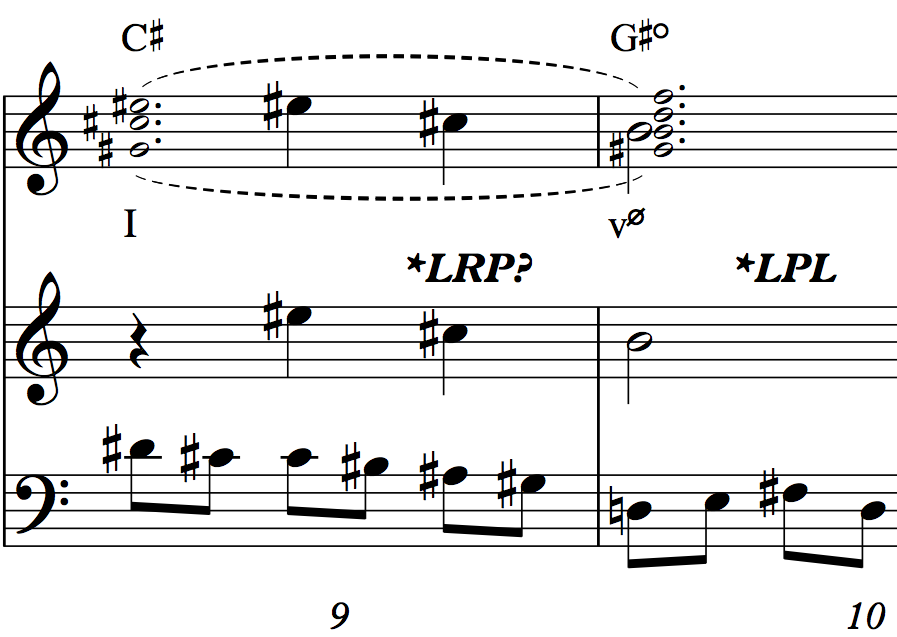
\includegraphics[width=\linewidth]{STTMP_m9-10}
\caption{ST:TMP Overture m. 9-10}
\label{fg:sttmp_m.9-10}
\end{marginfigure}

